\section{Empirical Force--Field model}
\label{sec:EmpiricalFF}
As we have seen in the previous section \ac{MD} provides a variety of tools for solving the time evolution of a $N$--particles system to obtain its dynamics. Due to the possibility to capture different length and time scales \ac{MD} simulations can be used in a variety of systems, such as set of atoms, molecules or more complex system such as protein and macromolecules systems. In each of these systems, depending on the \textit{interaction model} and its \textit{parametrization}, we will be able to describe crucial molecular--level processes, such as hydrogen bond formation in organic molecules, which happen on the picoseconds time scale; or study slow processes such as the diffusion of massive colloidal particles, taking place on time scales of milliseconds if not seconds.
When we study a soft or condensed matter system or, in general, a system composed by a large number of atoms (of the order of $N \gg 1000$), a crucial role is played by the \textit{Born--Oppenheimer approximation}. It says that we can separate the motion of the electrons by the motion of the atomic nuclei. That is done for integrating out the high frequency electrons' motions in order to remove some \ac{DOF}. Moreover the main interesting processes of soft and condensed matter, ranging from protein folding to glass transitions, from surface diffusion to ligand--receptor binding take place on longer time scales and involve larger number of atoms. Further if we want to know precisely the dynamics of the electrons in the system we have to introduce quantum mechanical methods that are, even for a small number of particles (of the order of $N\sim 100$), to much computationally time consuming, thus the Born--Oppenheimer approximation is indispensable. In the following, when we speak about atoms or chemical moieties we refer to it as for nuclei coordinates only without considering electrons at all.

Nevertheless atoms or molecules interactions, such as bond formation, are mediated by the electrons interactions.
Thus, to describe the dynamics of such a system with a classical \ac{MD} tools and the Born--Oppenheimer approximation, it is necessary to develop an \textit{empirical model of the inter--atoms interactions} that mimic correctly the ``real'' interactions. Since forces are derived from the \ac{PEF} we need a model composed by the set of the simplest pairwise addictive potentials that mimic the inter--particles interactions.
The model, the set of simulation parameters, such as the time step, the set of functional forms of the inter--particles interactions potential and its parameterizations are collected into the so called empirical \acf{FF}.
The meaning of \textit{empirical} is that most of the functional forms of the inter--atoms interaction has no ``first principle'' justification and they are only an approximation to reality: There is not a correct expression of them and they are chosen as a compromise between accuracy and computational efficiency. Further it is necessary to stress out that a \ac{FF} is a well defined single entity containing the simulation parameters, the functional models of the interactions and also its parameterizations (and the way to obtain it). All the parameters of a \ac{FF} are in harmony to each other thus changing some parameters without retesting whole \ac{FF} is not allowed because, maybe, one can destroy the whole \ac{FF}.

For biomolecular applications two main classes of \acp{FF} exist: The \textit{atomistic} \acp{FF} in which basic particles are atoms, and the \textit{coarse--grained} \acp{FF} in which the basic particles represent atom groups or small chemical moieties. In this case, even the way to do the corse--graining of the atoms in the molecules, called \textit{mapping}, is part of the \ac{FF} itself. Different \ac{CG} \acp{FF} can use different mapping methods even with the same functional forms. In the following we will add some other information about \acp{FF} and describe the principal functional forms for modeling the inter--particles interactions and how to treat them in a \ac{MD} simulation. While in the next section we will focus on the main \ac{CG} \ac{FF} used in this thesis work: The \textacr{MARTINI} \ac{CG} \ac{FF} developed by Marrink \etal\, \cite{Martini}.

\paragraph{\textbf{\textacr{parameterization}}} In general the functional forms for potential interactions are common to all particles in the system, then the \ac{FF} is completed by a set of empirical parameters that characterize the interaction between different types of particles, whether they are atoms or whole chemical groups.
Interaction parameters are empirical in the sense that they are assigned to reproduce a small set of target properties on a small group of systems. These target properties can be derived from experimental measurements or from finer--level calculations or simulations. Nowadays, atomistic and \ac{CG} biomolecular \acp{FF} come as ``packages'' of parameters and functional forms appropriate for the description of a large variety of chemical compounds in the liquid and solid phases.

\paragraph{\textbf{\textacr{transferability}}} As described above the parameterization of a \ac{FF} involves a small set of test systems for which some set of target proprieties are reproduced. The main characteristic of a \ac{FF} is the \textit{transferability} that means the ability of the model to describe different situations that differ from those used at the parameterization stage. Of course one would expect to be able to make some predictions for a bigger variety of systems and for other proprieties not used in the parametrization stage. Common faults of organic \acp{FF} concern, for example, phase transitions of organic compounds and phase transitions temperatures.

\subsection{Inter--particles interactions}
For biomolecular applications the inter--particles interaction potentials are divided into two main classes: The \textit{bonded interactions} involving particles within the same molecules and the \textit{non--bonded interactions} engaging all particles in the system and which usually represent the Van der Waals and the electrostatic interactions. The most common and general functional form for the \ac{PEF} is the following one
\begin{equation}
	\begin{aligned}
		U(\vec r_1, \cdots \vec r_N) = &\quad \frac{1}{2}\sum_{\text{bonds}} \frac{1}{2}k_i^b(l_i - l_{i0})^2\ + \frac{1}{2}\sum_{\text{angles}} k_i^a (\theta_i - \theta_{i0})^2\ +\\
		&+ \frac{1}{2}\sum_{\text{torsions}} V_n(1+\cos (n\omega - \gamma))\ + \\
		&+ \sum_{i=1}^N \sum_{j>i} \left ( {4\epsilon_{ij} \left ( \left ( \frac{\sigma_{ij}}{r_{ij}} \right )^{12} - \left ( \frac{\sigma_{ij}}{r_{ij}} \right )^6 \right )  + \frac{q_iq_j}{4\pi\varepsilon_0 r_{ij}}} \right )
	\end{aligned}
	\label{eq:FFPEF}
\end{equation}
The first two terms in equation~\eqref{eq:FFPEF} are harmonic potentials which model respectively the energy contribution due to deviation from reference bond length $l_{i0}$ and bond angle $\theta_{i0}$. Together with the bond and angle elastic constants, $k_{bi}$ and $k_{ia}$ respectively, they constitutes the set of parameters for bond and angle contributions. The angle contribution involves a set of three particles in the same molecule.  The middle line of equation~\eqref{eq:FFPEF} concerns the energy contribution due to the bond torsional change where $\omega$ is the
torsional angle. It involves four particles in the same molecule and mimic the energy barrier needed to rotate the bond angle along the bond axis. $\gamma$ is a phase factor, $V_n$ qualitatively describes the energy barrier for each $n$--th components and $n$ is defined as the number of minima for each components. The last line in equation~\eqref{eq:FFPEF} contains the energy contribution due to the non--bonded interactions: the Van der Waals modeled by a Lennard--Jones $12-6$ potential, fully characterized by the constants $\sigma_{ij}$ and $\epsilon_{ij}$ proper for each particles pair; and the electrostatic potential described by the particles charge $q$. The non--bonded interactions involve obviously all particles in the system, but for particles belonging to same molecule they are computed only if they  are separated by at least three bonds, i.e. if their interactions are not described by bonded terms. The various contributions described above are schematically represented in figure~(\ref{fig:FFInteraction}).

\begin{figure}[!ht]
	\centering
	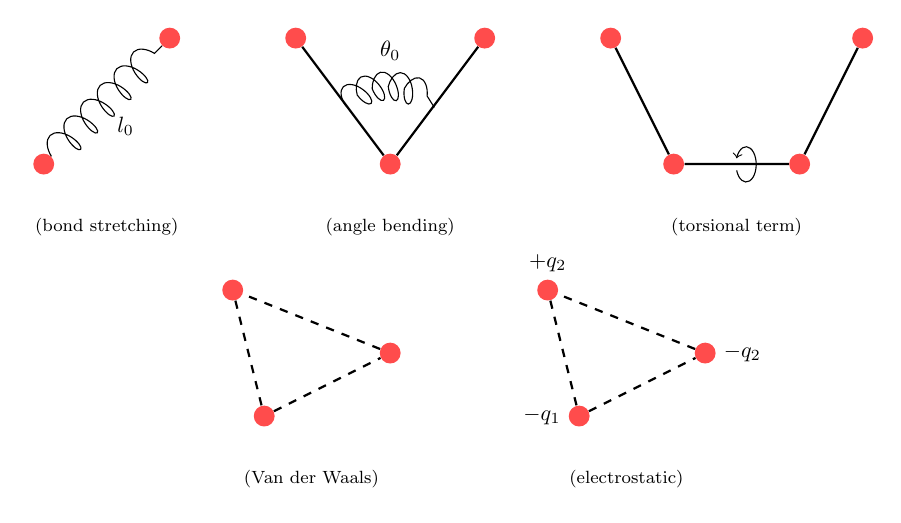
\begin{tikzpicture}[scale=0.8,transform shape]
		%\draw[thin, gray!25] (0,0) grid (15,8);
		\node[fill=red!70, circle, radius=0.15] (1) at (0,6) {};
		\node[fill=red!70, circle, radius=0.15] (2) at (2,8) {};
		\draw[decorate, decoration={coil,segment length=3mm,amplitude=2mm}] (1) -- (2);
		\node[] at (1.3,6.6) {$l_0$};
		\node[] at (1,5) {\footnotesize(bond stretching)};
		\node[fill=red!70, circle, radius=0.15] (3) at (4,8) {};
		\node[fill=red!70, circle, radius=0.15] (4) at (5.5,6) {};
		\node[fill=red!70, circle, radius=0.15] (5) at (7,8) {};
		\draw[thick,-] (3) -- (4) node[midway] (mid1) {};
		\draw[thick,-] (4) -- (5) node[midway] (mid2) {};
		\draw[-,decorate, decoration={coil,segment length=2mm,amplitude=2mm}] (4.8,6.91924) to[out=45,in=135] (6.2,6.9);
		\node[] at (5.5,7.8) {$\theta_0$};
		\node[] at (5.5,5) {\footnotesize(angle bending)};
		\node[fill=red!70, circle, radius=0.15] (6) at (9, 8) {};
		\node[fill=red!70, circle, radius=0.15] (7) at (10, 6) {};
		\node[fill=red!70, circle, radius=0.15] (8) at (12, 6) {};
		\node[fill=red!70, circle, radius=0.15] (9) at (13, 8) {};
		\draw[thick,-] (6) -- (7);
		\draw[thick,-] (7) -- (8);
		\draw[thick,-] (8) -- (9);
		\draw[->] (11,5.9) arc [start angle=-160, end angle=160, x radius=0.16cm, y radius=0.28cm];
		\node[] at (11,5) {\footnotesize (torsional term)};
		\node[fill=red!70, circle, radius=0.15] (10) at (3,4) {};
		\node[fill=red!70, circle, radius=0.15] (11) at (3.5, 2) {};
		\node[fill=red!70, circle, radius=0.15] (12) at (5.5, 3) {};
		\draw[thick,dashed] (10) -- (11);
		\draw[thick,dashed] (11) -- (12);
		\draw[thick,dashed] (12) -- (10);
		\node[] at (4.25,1) {\footnotesize(Van der Waals)};
		\node[fill=red!70, circle, radius=0.15, label=above:$+q_2$] (13) at (8,4) {};
		\node[fill=red!70, circle, radius=0.15, label=left:$-q_1$] (14) at (8.5, 2) {};
		\node[fill=red!70, circle, radius=0.15, label=right:$-q_2$] (15) at (10.5, 3) {};
		\draw[thick,dashed] (13) -- (14);
		\draw[thick,dashed] (14) -- (15);
		\draw[thick,dashed] (15) -- (13);
		\node[] at (9.25,1) {\footnotesize(electrostatic)};
	\end{tikzpicture}
	\caption{Schematic representation of the common inter--atoms interactions for biomolecular applications: bond stretching, angle bending, torsional term, Van der Waals and electrostatic interactions.}
	\label{fig:FFInteraction}
\end{figure}

\subsection{Non--bonded interactions}
\label{sec:nonbonded}
The bonded interactions, as we can see in equation~\eqref{eq:FFPEF}, are at \textit{fixed range}, meaning that they depend, for example, on the equilibrium bond length that is fixed. The same does not hold for the non--bonded interactions because they depend on the inter--particles distance $r_{ij}$ and they decay to zero as a power of $r_{ij}^{-d}$. Depending on the power order $d$ compared to the dimensionality $s$ of the system they are split into \textit{short range} if $d>s$ and \textit{long range} interactions if $1 \le d < s$. For example, as we shall see later, the Lennard--Jones $12-6$ potential decays to zero as $r^{-6}$ then it is a short range interaction, while the electrostatic is a long range interaction since it decays to zero as $r$.

\subsubsection{Cut--off, shift and switch methods}
As we have mentioned in~\ref{sec:neighbor} the calculations of the non--bonded interactions energy contributions is one of the most time consuming part of an \ac{MD} simulations. Since they are pairwise interactions their calculation scale as $\sim N^2$. Especially for the short range interactions, various methods were developed in order to speed--up the simulations. The \textit{cut--off} method is the most used to treat the short range interactions and, in same cases, even the long range one. Obviously this is strictly connected to the way neighbor list are computed as we have seen a cut--off method alone is not enough to speed up the simulation. Taking one particle into account, the general idea is to evaluate the non--bonded interactions with all other particles that are closer to the first for a distance $r_c$, called \textit{cut--off} radius, otherwise the interactions is set to $0$. This means that the new potential is of the form
\begin{equation*}
v^*(r) = \left \{
	\begin{aligned}
&v(r) & \quad & r \le r_c \\
&0    & \quad & r >   r_c
	\end{aligned} \right .
\end{equation*}

This generates a discontinuity in the potential and in its first derivative, i.e. in the forces: This is bad for energy conservation. A trick for solving the discontinuity of the potential and to improve the energy conservation is to apply also a \textit{shift} of the potential value at $r_c$, since it is a constant it does not affect the forces. We have
\begin{equation*}
v^*(r) = \left \{
	\begin{aligned}
&v(r) - v(r_c) & \quad & r \le r_c \\
&0    & \quad  & r >   r_c
	\end{aligned} \right .
\end{equation*}
Moreover to solve the discontinuity of the forces, that can cause some instability in a simulation, we need to consider a linear term proportional to the first derivative of the potential, such as
\begin{equation*}
v^*(r) = \left \{
	\begin{aligned}
&v(r) - v(r_c) - \left . \frac{dv(r)}{dr}\right |_{r_c}\ (r - r_c) & \quad & r \le r_c \\
&0    & \quad  & r >   r_c
	\end{aligned} \right .
\end{equation*}
Although, the shift methods make the potential quite different from the ``true'' one and this makes difficult to retrieve the correct thermodynamics proprieties. Thus, even if it can solve some instabilities, it must be carefully used.

Another powerful method is the \textit{switch} method. The general idea is to consider two cut--off radii  $r_{c1}$ and $r_{c2}$. If $r \le r_{c1}$ the ``true'' forms are used; while for $r > r_{c2}$ the potential is set to zero. For $r_{c1} < r \le r_{c2}$ a \textit{switching function} is considered in order to \textit{smoothly} switch the potential to zero.

It is important to stress out that even the method used to treat the interactions, as the cut--off radii and eventually the switching function, are part of the simulation parameters that are still part of the \ac{FF}. So they are interdependent with the model parameterizations, and should never be changed without retesting some target properties.


\subsection{Van der Waals interactions}
Van der Waals forces are a set of interactions that are divided into two main contributions: an attracting interaction and a repulsive one. The main contribution to both is due to quantum dynamics effect of the electron cloud interactions through the Pauli exclusion principle and to the instantaneous electrostatic interactions, even if both atoms are neutral, such as dipole--dipole, induced dipole--dipole and induced dipole--induced dipole interactions which, in a more rigorous description should be treated quantum mechanically. Both London dispersion forces, involving polar and non-polar atoms and related to instantaneous multipoles interactions, and hydrogen bonding, due to quantum effects, instantaneous electrostatics interactions and entropy effects, contribute to the attractive part of the potential. 
%To the attractive contribution there are also the London dispersion forces that involves polar and non--polar atoms and is due to the instantaneous multipoles interactions, and the hydrogen--bonding that is due to quantum effect, instantaneous electrostatic interactions and an entropic contribution.

The usual model to treat Van der Waals interactions is a Lennard--Jones potential. The most common exponents for the attractive and repulsive contributions to the potential are $6$ and $12$, respectively, although $6$ and $9$ can also be found depending on the system. The general form for a $12-6$ Lennard--Jones potential is the following
\begin{equation}
	v(r) = 4\epsilon\left ( \left ( \frac{\sigma}{r}\right )^{12}  - \left ( \frac{\sigma}{r} \right )^6 \right ) = \frac{C_{12}}{r^{12}} - \frac{C_{6}}{r^{6}}
	\label{eq:lj126}
\end{equation}
where $C_{12} = 4\epsilon\sigma^{12}$, $C_{6} = 4\epsilon\sigma^{6}$ and $r$ is the pairwise particles distance. $\epsilon$ is related to the absolute value of minimum while $\sigma$ is relented to the position of the minimum of the potential: $r_{\text{min}} = 2^{\nicefrac{1}{6}}\sigma$, often referred to by Van der Waals radius. These constants are proper for each particle pair. The attractive contribution is due to the negative part proportional to $r^{-6}$ while the repulsive one is due to the positive part proportional to $r^{-12}$. In figure~(\ref{fig:LG12511}) there is a example plot of the function~\eqref{eq:lj126} with $\epsilon = \sigma = 1$.
\begin{figure}[!ht]
\centering
	\begin{tikzpicture}
		\begin{axis}[samples=1000,domain=0:3,restrict y to domain =-2:2,axis x line=bottom,axis y line=center,xlabel={$r$},xmin=0,ymin=-1.5,ymax=1.5,xmax=3,ytick={-1.5,-1,...,1.5}]
			\addplot[very thick]plot (\x,{4/\x^(12)-4/\x^(6)});
			\addplot[dashed]plot (\x, {0});
		\end{axis}
		\node[] at (-1.4,3) {$v(r)$};
	\end{tikzpicture}
	\caption{Example plot of a Lennard--Jones function with $\epsilon = \sigma = 1$.}
	\label{fig:LG12511}
\end{figure}

The simplest and computationally most efficient way to treat a Lennard--Jones function, and in general all the short range interactions, is to use the cut--off method together with the shift or switch methods in order to obtain a continuous potential and/or a continuous forces. As we can see from figure~(\ref{fig:LG12511}) the Lennard--Jones potential go to zero rapidly with distance: at $r \sim 2\sigma$ its value is less then $1\%$ of the value in $r \sim \sigma$. A good choice for the cut--off is then of the order of $r_c \sim 2\sigma \div 3\sigma$.

\subsection{Electrostatic interactions}
\label{sec:longRangeInt}
One of the most important long range interaction is the electrostatic one. Despite the long range characteristic, for purely computational efficient reason, most of the \acp{FF} for biomolecular applications treat them in the same way as a short range interaction by a cut--off method\footnote{In general, for computational reason, a common choice is to consider the some cut--off for Van der Waals and electrostatic interactions.}. Of course this is an approximation and can lead to a serious issues in those proprieties or systems that strongly depend on the electrostatic interaction. Most issues due to a bad treatment of the Coulomb interactions are related to the development of a good polar solvent model (a good treatment of the electrostatic proprieties of water is really important for biological applications), as well as to the study of the interactions of charged particles with polar solvents, transport processes of charged moieties, calculations of the electrostatic potential inside macromolecules and so on. The loss of computational efficiency in the calculations of the electrostatic energy contribution is that it needs to take into account \textit{all particles} in a system, but we can not forget \ac{PBC}: even all the infinity images of all particles need to be taken into account.

If we consider only the simulation box the energy contribution is
\begin{equation}
	U = \frac{1}{2}\sum_{i=1}^N\sum_{j\ne i}^N\frac{1}{4\pi\varepsilon_0}\frac{q_iq_j}{r_{ij}}
	\label{eq:electrostatic}
\end{equation}
where $q_i$ and $q_j$ are the charge of particles $i$ and $j$, respectively, and $r_{ij}$ is the distance between $i$ and $j$. But we need also all image boxes. Supposing, for simplicity, that the box is a cube of size $L$, then we can define a tern of integer numbers $(n_x,\ n_y,\ n_z)$, $n_i=0,1,2,\cdots$ so that the position of all other image boxes, with respect to the central simulation box, is $\vec n = L (n_x,\ n_y,\ n_z)$. Then the energy contribution becomes
\begin{equation}
	U = \frac{1}{2}\ \sideset{}{'}\sum_{n_x,n_y,n_z}^{+\infty}\ \sum_{i=1}^N\sum_{j=1}^N\frac{1}{4\pi\varepsilon_0}\frac{q_iq_j}{\|\vec r_i - \vec r_j + \vec n \|}
	\label{eq:electrostaticImage}
\end{equation}
where the prime indicates that for $\vec n = 0$, i.e. the energy contribution of the simulation box, we need to exclude the self interaction term: So in inner sum it must be $j \ne i$.

As described above, a cut--off method is a good easy way to solve equation~\eqref{eq:electrostatic} and sometimes it produces good results. However, the increasing of computer power can lead to develop more rigorous methods to solve equation~\eqref{eq:electrostaticImage}, even for very large systems. The main problem is that the summation in equation~\eqref{eq:electrostaticImage} is \textit{conditionally convergent}\footnote{A conditionally convergent series contains both positive and negative terms such that the positive or negative term alone form both a divergent series. The sum of a conditionally convergent series depends on the order in which the positive and negative terms are considered.} and converges extremely slowly so that it would need so many terms to converge that its computational cost would be too high, especially for large systems (of the order of $N \sim 3\cdot 10^4$). The most important methods developed to solve this problem are based on the \textit{Ewald Summation Method} (\acs{ESM}). We shall describe those used in this thesis work: the \ac{ESM} itself and the \textit{Particle Mesh Ewald} (\acs{PME}) method. For a more complete discussion about the advanced methods developed to treat the electrostatic interactions for biological applications the reader is addressed to the Review by Cisneros \etal\, \cite{Cisneros}.

\subsubsection{Ewald summation method} %Molecular Modelling, 334
The \acf{ESM} is the first method introduced by Ewald
%L'articolo è in tedesco... Lo devo citare?, in realtà è citato nel Leach
for a correct treatment of the electrostatic energy contribution in an ionic crystal that can be modeled as the electrostatic interactions of a periodic charge density. The basic idea is to split the summation in equation~\eqref{eq:electrostaticImage} in two series both rapidly convergent. The method is based on the following identity
\begin{equation}
	\frac{1}{r} = \frac{f(r)}{r} + \frac{1 - f(r)}{r}
	\label{eq:ewaldTrick}
\end{equation}
the trick is to choose a function $f(r)$ that will deal with the rapid variation of the $1/r$ term for small $r$ and the slow decay at long $r$; in that case the two series can rapidly converge.

\begin{figure}[!hb]
	\centering
	\subfloat[Real space]{%
		\begin{tikzpicture}[scale=0.8, transform shape]
			\begin{axis}[samples=1000,domain=-1:4,axis x line=center,axis y line=none,axis x line=none, xmin=-0.4,xmax=2.5,ymin=-2.5, ymax=2.5]
				\addplot[thick]plot (\x, {0});
				\addplot[]plot (\x, {exp(-9*\x*\x/0.1)});
				\addplot[]plot (\x, {exp(-9*(\x-2)^2/0.1)});
				\addplot[]plot (\x, {-exp(-9*(\x-1)^2/0.1)});
				\addplot[smooth] plot coordinates {(0,0) (0,-1.5)};
				\addplot[smooth] plot coordinates {(1,0) (1,1.5)};
				\addplot[smooth] plot coordinates {(2,0) (2,-1.5)};
			\end{axis}
		\end{tikzpicture}
	}%
	\qquad
	\subfloat[Reciprocal space]{%
		\begin{tikzpicture}[scale=0.8, transform shape]
			\begin{axis}[samples=1000,domain=-1:4,axis x line=center,axis y line=none,axis x line=none, xmin=-0.4,xmax=2.5,ymin=-2.5, ymax=2.5]
				\addplot[thick]plot (\x, {0});
				\addplot[]plot (\x, {-exp(-9*\x*\x/0.1)});
				\addplot[]plot (\x, {-exp(-9*(\x-2)^2/0.1)});
				\addplot[]plot (\x, {exp(-9*(\x-1)^2/0.1)});
			\end{axis}
		\end{tikzpicture}
	}%
	\caption{Schematic illustration of the \acl{ESM} charge distribution: in (a) point charges (represented by vertical lines) and the neutralizing Gaussian charge distribution; in (b) the counteracts Gaussian distribution.}
	\label{fig:ewald}
\end{figure}

The \ac{ESM} for electrostatic interactions works, as illustrated in figure~(\ref{fig:ewald}), considering each point--like charge in the system surrounded by a neutralizing charge distribution of equal magnitude but opposite sign that decays rapidly to zero. Simplifying the notation for a one dimensional system, the simplest functional form is a Gaussian distribution centered in the position $r_i$ of the point--like charge $q_i$, of the form
\begin{equation}
	\rho_i(r) = \frac{q_i\alpha^3}{\pi^{3/2}}e^{-\alpha^2 (r - r_i)^2}
\end{equation}
that obeys the relation
\begin{equation*}
	\frac{q_i\alpha^3}{\pi^{3/2}}\int_{r_i-\epsilon}^{r_i+\epsilon}e^{-\alpha^2 (r - r_i)^2}\ dr \simeq q_i
\end{equation*}
where $(r_i-\epsilon; r_i+\epsilon)$ is a small interval around $r_i$. The energy contribution due to this set up, the point--like charge \textit{and} the gaussian charge distribution, is given by
\begin{equation}
	U_r = \frac{1}{2}\sum_{i=1}^N\sum_{j=1}^N\ \sideset{}{'}\sum_{n_x,n_y,n_z}\ \frac{q_iq_j}{4 \pi \varepsilon_0} \frac{\erfc{(\alpha \| \vec r_i - \vec r_j + \vec n \|)}}{\| \vec r_i - \vec r_j + \vec n \|}
	\label{eq:ewaldReal}
\end{equation}
where $\erfc{(x)} = 1-\erf{(x)}$ is the complementary error function and $\erf{(x)}$ is the error function. They are given by
\begin{equation}
	\erfc{(x)} = \frac{2}{\sqrt{\pi}}\int_{x}^{+\infty} e^{-t^2}\ dt, \qquad \erf{(x)} = \frac{2}{\sqrt{\pi}}\int_{0}^{x} e^{-t^2}\ dt
	\label{eq:erf}
\end{equation}

The point is that the summation involving the complementary error function in equation~\eqref{eq:ewaldReal} is rapidly convergent and it needs very few terms so that a cut--off method can be safely used. The rate of convergence depends on the $\alpha$ parameter, the bigger is $\alpha$ the more rapidly converge and the shorter can be the cut--off radius.
Thus the \ac{ESM} use the $\erfc{(r)}$ as $f(r)$ function in equation~\eqref{eq:ewaldTrick}. Of course since we added a non physical neutralizing charge in the system, in order to restore the real charge distribution, we must consider another distribution, called counteracts charge distribution, of equal magnitude but opposite sign. Considering the identity in equation~\eqref{eq:ewaldTrick} this lead to an energy contribution of the form $(1-f(r))/r$, so, using equation~\eqref{eq:erf}, it is of the form $\erf{(r)}/r$. Another trick is to compute the former in the \textit{real space}, the latter in the \textit{reciprocal space}, thus considering its Fourier transform. This energy contribution is given by
\begin{equation}
	U_f = \frac{1}{2}\sum_{i=1}^N\sum_{j=1}^N\ \sum_{k_x,k_y,k_z}\ \frac{1}{4\pi\varepsilon_0}\frac{4\pi}{L^3k^2}e^{-k^2/(4\alpha^2)}e^{\mathsf{i}{\vec k \cdot (\vec r_i - \vec r_j)}}
	\label{eq:ewaldReciprocal}
\end{equation}
where $\vec k = 2\pi\vec n/L$ are the reciprocal lattice vectors. Even $U_f$ converges rapidly as $U_r$ in equation~\eqref{eq:ewaldReal}; then a cut--off method can be safely used. Nevertheless, as opposite to $U_r$, the smaller is $\alpha$ the shorter can be the cut--off. Clearly a proper \textit{balance} between the real and reciprocal space summation is needed.

Since in equation~\eqref{eq:ewaldReal} even the self interaction with each Gaussian is included we need to add another item for cancel it out; this is done by the self--term
\begin{equation}
	U_{self} = -\frac{\alpha}{\sqrt{\pi}}\sum_{i=1}^N\frac{q_i}{4\pi\varepsilon_0}
	\label{eq:EwaldselfTerm}
\end{equation}

Summarizing, the energy contribution of the electrostatic interactions by the \ac{ESM}, is computed summing equations~\eqref{eq:ewaldReal},\eqref{eq:ewaldReciprocal} and~\eqref{eq:EwaldselfTerm} to obtain
\begin{equation}
	\begin{aligned}
		U =&\quad\frac{1}{2}\sum_{i=1}^N\sum_{j=1}^N\ \sideset{}{'}\sum_{n_x,n_y,n_z}\ \frac{q_iq_j}{4 \pi \varepsilon_0} \frac{\erfc{(\alpha \| \vec r_i - \vec r_j + \vec n \|)}}{\| \vec r_i - \vec r_j + \vec n \|}\ + \\
		 &+ \frac{1}{2}\sum_{i=1}^N\sum_{j=1}^N\ \sum_{k_x,k_y,k_z}\  \frac{1}{4\pi\varepsilon_0}\frac{4\pi}{L^3k^2}e^{-k^2/(4\alpha^2)}e^{\mathsf{i}{\vec k \cdot (\vec r_i - \vec r_j)}}\ + \\
		 &- \frac{\alpha}{\sqrt{\pi}}\sum_{i=1}^N\frac{q_i}{4\pi\varepsilon_0}
	\end{aligned}
	\label{eq:EwaldEnergy}
\end{equation}
The first line is the real space contribution while the second is the Fourier energy contribution. Since the last self--interaction term is constant it does not affect forces computation. The \ac{ESM} offers a well defined method to properly treat electrostatic interactions, nevertheless it is quite expensive in term of computational resources. If $\alpha$ and the cut--off are constant, then the computation scales as $\sim N^2$; while if $\alpha$ and the cut--off are dynamically updated it scales as $\sim N^{\nicefrac{3}{2}}$; this can lead to an incompatibility between the Van der Waals interactions cut--off and the electrostatic one thus compromising the efficiency gain. Despite we have described \ac{ESM} applying it to the electrostatic interactions, it can be used, with some changes, with all long--range interactions and in general to all energy contributions that decay as $r^{-d}$, for example, even with the Van der Waals energy contribution.

For biomolecular applications most \ac{MD} tools set an equal cut-off radius for both Van der Waals interaction and the real part of the Ewald summation~\eqref{eq:EwaldEnergy} in order to achieve for both a scaling of the order $\sim N$. However in this way the computation of the reciprocal part in the Ewald summation~\eqref{eq:EwaldEnergy} will be very inefficient as it scales as $\sim N^2$. In order to increase the efficiency of the calculation of the Fourier transform various of advanced methods can be used. They are all based on the use of the \ac{FFT} method. In this way the reciprocal part can scale as $\sim N\ln N$. Since \ac{FFT} requires discretized quantities, the idea of such methods, called \textit{Particle Mesh} is to consider the charge density spread on a mesh grid and then evaluate the electrostatic potential via solving the Poisson's equation\footnote{Given a charge distribution $\rho(\vec r)$ then the associated electrostatic potential $\phi(\vec r)$ can be calculated solving the Poisson's equation $\displaystyle \nabla^2\phi(\vec r) = -\frac{1}{\varepsilon_0} \rho(\vec r)$. If a charge $q$ is at position $\vec r$ its electrostatic potential energy is given by $U = q\phi(\vec r)$.}
using fast Poisson solver together with the \ac{FFT} method; this can be done, for example, exploiting the \ac{PBC} in order to discretize and make periodic the Poisson's equation
%\footnote{It is generally true that the Poisson's equation become ``easily'' solvable in Fourier space. Considering a one dimensional Poisson's equation, its Fourier transform is $k^2\varepsilon_0\tilde\phi(k) = \tilde \rho(k)$ where $\tilde\phi(k)$ and $\tilde\rho(k)$ are, respectively, the Fourier transform of the electrostatic potential and charge distribution.}.
Such algorithms include the \textit{particle--particle particle--mesh} method, \textit{Particle mesh Ewald} method, \textit{Fast--Fourier Poisson} method and a recent methodology based on multi--scale mesh grid; the efficiency and accuracy of such mesh--based algorithms depends strongly on the way in which the charges are attributed to mesh points, this makes the methods different. In the following we will describe the one used in this thesis work, the \acf{PME} method.

\subsubsection{Particle mesh Ewald method}
\acf{PME} method developed by Darden \etal\, \cite{DardenPME} is based on the \ac{ESM} so that the starting point is equation~\eqref{eq:EwaldEnergy} in which, as described above, the first part of the Ewald summation is computed in the real space together with the Van der Waals contribution using the same cut--off radius while the reciprocal part is computed using \ac{FFT} method, in order to have a gain of performance. To do this, first, we need to consider a grid mesh onto which the Gaussian counteracts charge distribution is spread. The basic idea, then, is to calculate the electrostatic energy solving Poisson's equation through \ac{FFT} methods. The efficiency and accuracy depend on the way the charges are distributed onto the grid. To do this a \textit{charge assignment function}, $W(r)$ is introduced such that, considering for simplicity a one dimensional system, the fraction of a charge at position $r$ assigned to a grid point at position $r_p$ is given by $W(r_p - r)$. Hence, if we have a charge density $\rho(r)$ then the charges at the grid point $r_p$ are given by
\begin{equation}
	q_M(r_p) = \int_0^L\ W(r_p - r) \rho (r)\ dr
	\label{eq:meshAssign}
\end{equation}
where $L$ is the box length and, if $h$ is the grid spacing, $M = L/h$ is the number of mesh point. In figure~(\ref{fig:gidAssign}) the charges assignment is schematically represented. The assignment function should have the following proprieties: should be an even function and should be normalized in such a way that the sum of the fractional charges equals the total charge of the system. Moreover the best accuracy is obtained with a dense grid in order to reduce as much as possible the discretization of the charge density. However the computational cost increases as the number of grid points! So a balance between efficiency and accuracy is clearly needed.
\begin{SCfigure}
	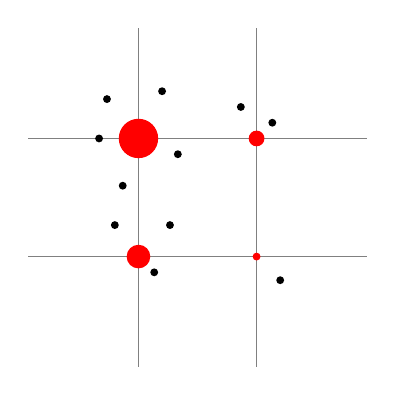
\begin{tikzpicture}
		\draw[gray,step=1.5] (0.1,0.1) grid (4.4,4.4);
		\fill[fill=red] (1.5,3) circle (0.25);
		\fill[fill=red] (3,1.5) circle (0.05);
		\fill[fill=red] (1.5,1.5) circle (0.15);
		\fill[fill=red] (3,3) circle (0.1);

		\fill[fill=black] (1, 3) circle (0.05);
		\fill[fill=black] (2, 2.8) circle (0.05);
		\fill[fill=black] (1.1, 3.5) circle (0.05);
		\fill[fill=black] (1.3, 2.4) circle (0.05);
		\fill[fill=black] (1.8, 3.6) circle (0.05);

		\fill[fill=black] (1.2, 1.9) circle (0.05);
		\fill[fill=black] (1.7, 1.3) circle (0.05);
		\fill[fill=black] (1.9, 1.9) circle (0.05);

		\fill[fill=black] (3.2,3.2) circle (0.05);
		\fill[fill=black] (2.8,3.4) circle (0.05);

		\fill[fill=black] (3.3,1.2) circle (0.05);
	\end{tikzpicture}
	\caption{A schematic representation of the charge assignment. The black filled circles are a unit particle charge, while the red ones, are the charges assigned to grid points. The bigger is the circle, the more is the charge.}
	\label{fig:gidAssign}
\end{SCfigure}

A nice way to solve the problem of charge assignment is to shift the problem to the discretization of the Fourier transform. This can be viewed as an interpolation problem. Consider the $e^{-\mathsf{i}\vec k\cdot \vec r_j}$ term in the Fourier transform of equation~\eqref{eq:ewaldReciprocal}. In general $\vec r_j$ does not correspond to a mesh grid point, so that term is not part of a discrete Fourier transform. The idea, thus, is to interpolate it in terms of values of the complex exponential at the mesh points. Switching for simplicity to a one dimensional system, if the mesh grid has $M = L/h$ points, a particle coordinate $r_j$ is located between mesh points $[r_j/h]$ and $[r_j/h] + 1$ where $[ ]$ denotes the integer part; thus a $p$--order interpolation of the exponential is of the form
\begin{equation*}
	e^{-\mathsf{i}kr_j} \simeq \sum_{i=1}^M W_{p}\left ( \frac{r_j}{h} - i \right ) e^{-\mathsf{i}khi}
\end{equation*}
where $W_{p}$ denotes the interpolation coefficient. A $p$--order interpolation means that only the $p$ mesh points nearest to $r_j$ contribute to the sum. Assuming a point--like charge distribution the Fourier transform of the charge density is therefore
\begin{equation*}
	\rho_k \simeq \sum_{i}e^{-\mathsf{i}khi} \sum_j\ q_iW_{p} \left ( \frac{r_j}{h} - i \right )
\end{equation*}
we can interpret the above expression as the discrete Fourier transform of the charge density
\begin{equation*}
	\rho(i) = \sum_j\ q_iW_{p} \left ( \frac{r_j}{h} - i \right )
\end{equation*}
but using equation~\eqref{eq:meshAssign}, it is nothing that the point--like charge distribution assigned to the mesh point $i$ through the assignment function $W_{p}$.

We clearly see that the charge assignment problem is now shifted to the complex exponential interpolation. There are two main methods to make the interpolation: the \textit{Lagrange interpolation method} and the \textit{Euler SPLINE interpolation method}. The basic idea of the former is to use, as interpolating function, a polynomial function of degree $ \le (n-1)$ where $n$ is the number of points to interpolate, that passes through all the $n$ points, and which is constructed with a summation over the \textit{Lagrange basis polynomials} as follow
\begin{equation*}
	P(x) = \sum_{i=1}^n y_i \prod_{\substack{k=1\\k\ne i}}^n \frac{x-x_k}{x_i - x_k}
\end{equation*}
where $(x_i;y_i)$ are the sets of points to interpolate. The main disadvantage of this method is that, even if $P(x)$ is continuous everywhere, its derivative is not, thus it can lead to some instability in \ac{MD} simulations. The latter method, that is the most used in \ac{MD} tools, is based on the concept of \textit{SPLINE interpolation}. Instead of using a unique interpolating function that passes through each point, the SPLINE method uses a \textit{piecewise polynomial function}, called SPLINE, in which each piece is smoothly connected and optimized to interpolate a subset of the points. The Euler SPLINE method use the \textit{exponential Euler SPLINE} that is constructed with the basis of the Euler $n$--degree polynomials $A_n(x;\lambda)$ generated by the following equation
\begin{equation*}
	\frac{\lambda - 1}{\lambda - e^z}e^{xz} = \sum_{n=0}^{+\infty} \frac{A_n(x;\lambda)}{n!}z^n
\end{equation*}
where $\lambda$ is a complex parameter and $z$ is a complex variable. The main properties of such SPLINE is that, it is $n-1$ times analytic, continuously differentiable and then can solve the instability problem of the Lagrange interpolation method. In literature the Euler SPLINE method is referred to as \textit{smooth} \acl{PME} and the reader is addressed to the article by Essmann \etal\, \cite{EssmannSPME} for more technical details about the interpolation procedure.

Summarizing, the \ac{PME} method is implemented with the following scheme
\begin{itemize}
	\item By the interpolation of the complex exponential in the Fourier transform of the Ewald summation, the Gaussian counteracts charge distribution are spread onto the mesh grid and a discretized Fourier transform is obtained;
	\item Poisson's equation for the discretized charges are solved through the \ac{FFT} methods;
	\item The reciprocal energy contribution is obtained considering the inverse Fourier transform;
	\item Electrostatic forces are computed and assigned to the charged system particles.
\end{itemize}
The main advantages of the \ac{PME} algorithm are that the potential energy and forces are smooth functions of the particles positions, offers a good energy conservations, offers a very well balance between accuracy and computational efficiency since it scales as $\sim N\ln N$ and it is easily generalizable to interaction potentials that decay as $r^{-d}$ such as the Lennard--Jones potential. Nevertheless it does not conserve very well the particles momentum due to \ac{RMS} errors in the forces calculations that have to be cancelled out by removing the forces averages.

\subsection{Charge representation}
\label{sec:chargeRep}
Even if some methods, such as the \ac{PME} one, have been developed to speed up the computation of electrostatic energy contribution one of the main problems of \acp{FF} for biomolecular applications which are related to the electrostatic interactions, remains the \textit{charge representation}: The way that the charges of atoms or molecules are assigned to the system particles. The problem arises from the necessity to represent the electrons clouds of atoms and molecules in the system an the interactions which they generate, that is, for instance a purely quantum effect. Nevertheless this is crucial for a better description of most electrostatic phenomena such as polarizability of molecules and polar solvent, solvation shell of charged ions, protein--ligands interaction, ion transport through polar and non--polar medium, self assembly processes and so on.

The mostly used solution is the \textit{atom--centered ``partial charge'' approximation} in which the full charge density of the molecule is replaced by fractional point--like charges assigned to each atom of the molecule. But now, one has to decide how much of the molecular charge density should be assigned to each atom. Traditionally most \acp{FF} assign each atom of a molecule a fixed partial--charge. The most used procedure for extracting partial--charges from molecular wave functions is based on fitting atomic charges with the molecular electrostatic potential, computed with \textit{ab initio} calculation such as \textit{density functional theory}. The fitting procedure consists in minimizing the deviation between the electrostatic potential produced by the assigned charge and the molecular electrostatic potential. Such representation is believed to be an important source of error in the electrostatics treatment. Moreover with fixed charge assignment it is more challenging to take into account those phenomena that involve a transfer of charge inside the molecule, as polarization effect. The use of off--centered charges and/or higher order atomic multipoles can significantly improve the treatment of electrostatics but of course it is necessary a good balance between accuracy and performances since the electrostatic problem can rapidly drive to a loss of efficiency sometimes without a really gain in accuracy.

\subsection{Polarization}
\label{sec:polarization}
Polarization refers to the redistribution of the electron charge density of a molecule in presence of an external electric field, generated, for example, by charged ions or another molecule. Polarization is responsible for non--addictive attractive inter-- or intra--molecular interactions which have many--body characteristics. Induced polarization effects should also be included. These effects have been recognized to have an important role in many biological interactions in which different compounds are present. An increasing number of studies show that the lack of these effects can lead to a serious limitations, particularly, for ionic systems and chemical process that involve different environments such us water and proteins or water and lipids. In \ac{MD} simulations polarization effects are included using either \textit{implicit} or \textit{explicit} methods.

The implicit method completely avoids the many--body calculation by including a mean polarization effect in the functional form of the interaction potential. The general idea is to surround all the simulation box by a transparent medium with a relative dielectric constant $\varepsilon_r$. In this way the polarization effect is taken into account considering a mean field theory and solving the Poisson's equation to determine the electrostatic potential due to system charges by the substitution $\varepsilon_0\rightarrow\varepsilon_0\varepsilon_r$. Since it avoids many--body calculations, this method gives an incomparable gain in performances bust it must be carefully used. The main disadvantage is that the mean polarization effect is added to all system particles and this wash out all the details about a possible polarization effect in a molecule, for example a protein or a piece of protein. This method can be safely used, for example, when our system is composed principally of one kind of solvent, for example water; but if the simulation box is composed of different chemical environments such as water and lipids or other organic compounds, using the same dielectric constant would lead to seriously incorrect results of the proprieties of the organic component and maybe affect the whole simulation.

The way to correct the above behavior is to use an explicit method. As the name suggests, the polarization effect is taken into account for every molecules in the system by a it proper model included in the \ac{FF}. The general idea is to add some more internal \ac{DOF} to a molecule or atom to take into account the movement of charges and/or split the point--like charge assigned, for example, to a chemical group, to a partial charge assigned to each particles of the chemical group itself. This can be done for every molecule or atom in the system and thus it is the optimum to better describe systems with different chemical environments.

%\subsection{Atomistic model}
\subsection{Coarse--Grained model}
\label{sec:CGModel}
As we have introduced at the beginning of this section, for biomolecular applications two main classes of \acp{FF} exist: atomistic \acp{FF} and \ac{CG} \acp{FF}. Since the atomistic model takes into account all the atoms in a molecule it is obviously the most real and accurate \ac{FF}. Nevertheless the number of \ac{DOF} of the system increases leading to a loss of performances. Moreover, basically, the atomistic \acp{FF} are efficient until the physical proprieties can be properly sampled on a time scale of a few microseconds over a length scale of a few nanometers. As the time and length scales increase more and more time is needed to carry out a complete simulation. Unfortunately many biological processes involving lipid membranes and other organic molecules, including synthetic compounds, take place on much longer time and length scales.

One possible solution is to \textit{integrate out} some \ac{DOF}, preserving those that are relevant for the problem in exam: this procedure is called \textit{coarse--graining}. The basic units of \ac{CG} \acp{FF} are called \textit{beads}, each representing a group of atoms or a well defined chemical moiety. The size of the group of atoms that is represented by a single bead determines the degree of coarsening of the \ac{FF}. Even in this case, all the general features described above, apply: functional forms need to be chosen and their parameterization need to be adjusted so as to reproduce the desired target properties. Moreover, in this case, even a \textit{mapping} procedure should be defined as the first step in the development of a \ac{CG} model: This establishes a link between the atomistic model and the coarse--grain beads. There is not a unique or correct procedure to obtain the mapping because it depends on the desired coarse--graining level, on the time and length scales that one wants to correctly sample and on the properties one wants to reproduce. For biological applications \ac{CG} \acp{FF} are often designed to reproduce specific thermodynamics properties such as surface tension, free energy of partitioning, free energy of hydration and so on, instead of, for example, the structural properties.

In general a \ac{CG} \ac{FF} is more computationally efficient than an atomistic one for the following reasons: the \ac{DOF} of the system are reduced due to the \ac{CG} procedure and a smaller number of interactions and forces has to be taken into account; bead--bead interactions, which result from the removal of finer structural details, are softer than atom--atom interactions. Thus, vibrational modes are slower, and their sampling can be achieved using larger \ac{MD} time steps than in atomistic simulations; softer interactions imply a smoother \ac{PEF} which leads to faster diffusion.

\section{MARTINI: a Coarse--Grained Force--Field}
\martini is a \ac{CG} \ac{FF} originally developed by Marrink \etal\, \cite{Martini} for organic solvents and lipids and then extended to proteins \cite{MartiniProtein}, carbohydrates \cite{MartiniCarbo} and a broad class of polymers \cite{MartiniPolymers}. The original aim was to improve the description of the physical and chemical properties of lipid membranes using a \ac{CG} model. The power of the model was immediately clear and soon its philosophy was changed to develop a \ac{FF} applicable to a broad range of organic system providing a set of extensively calibrated building blocks to construct a large variety of organic molecules without reparametrizing the \ac{FF}. This is possible, because, instead of focusing on accurately reproducing structural details of a particular system, the \ac{FF} is based on accurately reproducing the interaction between polar and non--polar chemical compounds. This is the main target property: The \textit{partitioning free energy} between water and a large number of organic solvents, i.e. the free energy of transfer of chemical moieties from polar and non--polar solvents. These building blocks are representative of the main chemical moieties in an organic system, this is the guide for the mapping procedure.

\subsection{Mapping}
The mapping of the \martini beads, is based on a four--to--one scheme that groups four heavy atoms like C, S, O and so on, plus their associated hydrogen atoms, into a single interaction site. Consistently four water molecules are modeled with one \martini bead. An example of the coarse-graining procedure including both atomistic and \ac{CG} descriptions is shown in figure~(\ref{fig:martiniMapping}).
\begin{figure}[!ht]
	\centering
	\includegraphics[width=0.6\textwidth]{img/martiniMapping}
	\caption{\martini mapping and atomistic structures compares of some molecules: (A) Standard water bead, (B) polarizable water bead, (C) \acs{DMPC} lipid, (D) Polysaccharide fragment, (E) Peptide, (F) \acs{DNA} fragment, (G) Polystyrene fragment and (H) Fullerene molecule. In all cases \martini \acs{CG} beads are shown as cyan transparent beads overlaying the atomistic structure. Taken from \cite{MartiniReview}.}
	\label{fig:martiniMapping}
\end{figure}

There are four main bead types: polar (P), non--polar (N), apolar (A) and charged (Q). Each bead type has a number of subtypes to take into account a more accurate representation of the chemical nature of the moieties due to underlying the specific atomistic structure. These subtypes are distinguished by the hydrogen bonding capabilities: donor (d), acceptor (a), both donor and acceptor (da) and none ($0$) and/or by their degree of polarity: lowest polarity ($1$), $\cdots$, highest polarity ($5$).

\begin{SCtable}\footnotesize
	\begin{tabular}{lc}
		\toprule
		Level  & $\epsilon$\,[kJ/mol] \\ \midrule
		O	   & $5.6$	 \\ \midrule
		I      & $5.0$	 \\ \midrule
		II	   & $4.5$	 \\ \midrule
		III	   & $4.0$	 \\ \midrule
		IV	   & $3.5$	 \\ \midrule
		V	   & $3.1$	 \\ \midrule
		VI	   & $2.7$	 \\ \midrule
		VII	   & $2.3$	 \\ \midrule
		VIII   & $2.0$	 \\ \midrule
		IX     & $2.0$	 \\ \bottomrule
	\end{tabular}
	\caption{Interaction strength parameter ($\epsilon$). The last one is for the special case $\sigma=0.62$~nm.}
	\label{tab:martiniEpsilon}
\end{SCtable}

\subsection{Interactions potential}
\paragraph{\textbf{van der waals interactions}} The functional form describing pairwise Van der Waals interaction is a Lennard--Jones $12-6$ potential as in equation~\eqref{eq:lj126}.
%The $\epsilon$ and $\sigma$ parameters are first obtained for a same--type interactions and then the inter--type parameters are computed as follow
%\begin{equation*}
%	\epsilon_{ij} = \sqrt{\esilon_{ii}\epsilon_{jj}} \qquad \sigma_{ij} = \frac{1}{2}(\sigma_{ii} + \sigma_{jj})
%\end{equation*}
For most beads the $\sigma$ parameter is set equal to $0.47~$nm except for the Q--C$_1$ and Q--C$_2$ interactions for which $\sigma = 0.62$~nm. This is consistent with reproducing the hydration shell when a charged bead (Q) is dragged into an apolar medium. The strength of the interactions is instead dived into ten levels, reported in table~(\ref{tab:martiniEpsilon}). The association of the interactions strength with the \martini beads is shown in figure~(\ref{fig:martiniInteractions}).
\begin{figure}[h!t]%
	\center
	\includegraphics[width=\textwidth]{img/martiniInteractions.pdf}%
	\caption{Interaction strength association matrix for the \martini bead types and subtypes. Taken from \cite{Martini}.}
	\label{fig:martiniInteractions}
\end{figure}

% \begin{adjustwidth}{-3cm}{-5cm}%
% \centering
% \begin{minipage}[c]{1.2\textwidth}%
% 	\includegraphics[width=\textwidth]{img/martiniInteractions.pdf}%
% 	\captionof{figure}{Interaction strength association matrix for the \martini bead types and subtypes. Taken from \cite{Martini}.}
% 	\label{fig:martiniInteractions}
% \end{minipage}
% \end{adjustwidth}

\paragraph{\textbf{electrostatic interactions}} Electrostatic charges are assigned using the atom--centered approximation, as described in~\ref{sec:chargeRep}. In this case, charges are no more fractional but are empirically assigned at the center of the beads trying to follow as much as possible the net charge of the associated chemical moieties. A special case is water, modeled as a P$_4$ bead, since it interacts only with Van der Waals interaction so that the polarizability effect is not very well described. To fill this lack it is used an implicit medium with a dielectric constant $\varepsilon_r = 15$. However, as we will see later in~\ref{sec:pw}, to avoid the problems with the implicit medium described in~\ref{sec:polarization}, especially for lipid membranes for which the dielectric constant in the hydrophobic region is much smaller, Yesylevskyy \etal\, \cite{PW} have developed a more sophisticated \ac{CG} water model, called \ac{PW}, to take into account a better water behavior.

\paragraph{\textbf{bonded interactions}} They includes only bond length and an angle harmonic contributions. The former is modeled with a harmonic potential as the first term in equation~\eqref{eq:FFPEF}, with the same bond constant for all bead types: $k^b = 1250$~kJ/(mol\ nm$^2$) and an equilibrium distance of $l_0 = 0.47$~nm. The later is modeled as a cosine--type harmonic potential
\begin{equation*}
	U = \frac{1}{2}k^a (\cos(\theta) - \cos(\theta_0))^2
\end{equation*}
whose parameters are: $k^a = 25$~kJ/mol and $\theta_0 = 180^\circ$ for aliphatic chains; $k^a = 45$~kJ/mol and $\theta_0 = 120^\circ$ for \texttt{cis} double bonds and $k^a = 45$~kJ/mol and $\theta_0 = 180^\circ$ for \texttt{trans} unsaturated bonds. Moreover, especially for ring systems, an improper dihedral angle harmonic potential can be used to prevent out of plane distortion. The form is
\begin{equation*}
	U = k_{id} (\theta_{ijkl} - \theta_0)^2
\end{equation*}
where $\theta_{ijkl}$ denotes the angle between the planes described by atoms $i,j,k$ and $j,k,l$; $k_{id}$ and $\theta_0$ are, as usual, the force constant and equilibrium angle.

\subsection{Simulation parameters}
\martini \ac{FF} was originally developed using a shifted cut--off scheme for both Lennard--Jones and electrostatic potentials with a cut--off radius $r_c = 1.2$~nm. The Lennard--Jones potential was shifted from $r_s = 0.9$~nm to $r_c$ while from $r_s = 0.0$~nm to $r_c$ for the electrostatic potential. The neighbor list is constructed as described in the first part of~\ref{sec:neighbor} with a refresh rate of $10$ \ac{MD} steps. Recently the more efficient Verlet cut--off scheme was tested by Marrink \etal\, \cite{MartiniReview} and used with the \martini \ac{FF} with a cut--off radius of $r_c = 1.1$~nm, a Verlet buffer tolerance of $0.005$~kJ/(mol$\cdot$ps) and a minimum refresh rate of $10$ \ac{MD} steps (often, depending on the hardware, it can be dynamically increased to $30$ or $40$ \ac{MD} steps getting better performances).  Moreover, the treatment of the electrostatic interaction can be safely updated to the \ac{PME} method together with the Verlet cut--off scheme. This new set--up was largely tested by Yesylevskyy \etal\, \cite{PW}. In this case the cut--off radius was set to $r_c = 1.2$~nm with the same Verlet buffer tolerance; the \ac{PME} grid spacing was set to have a lower bound of $0.12$~nm and the interpolation was set to a fourth-order. Moreover, with the use of \ac{PW}, as we shall see, the dielectric constant should be reduced to $\varepsilon_r = 2.5$. In all cases a time step up to $40$~fs is suitable for a great number of applications, but $20$~fs is the most powerful choice in terms of performance and accuracy balancing. It should be clear that changing these simulation parameters must be followed by a retest of the main properties of the \martini \ac{FF}.

\subsection{Parametrization}
In order to parametrize the \martini \ac{CG} \ac{FF} a set of thermodynamics properties, obtained from \ac{MD} simulations are compared and fitted against those experimentally measured. These properties are the \textit{free energies of vaporization}, \textit{hydration} and \textit{partitioning} between water and a set of organic compounds such as hexadecane (H), chloroform (C), ether (E) and octanol (O). The free energy of hydration was obtained from the partitioning of \ac{CG} compounds between bulk water in equilibrium with its vapor. Similarly the free energy of vaporization was obtained considering a simulation box with the selected \ac{CG} compounds in equilibrium with their vapor. From the equilibrium densities of the particles in both the phases the related free energies can be computed from
\begin{equation*}
	\Delta G = k_B T\ln \left ( \frac{\rho_{\text{vap}}}{\rho_{\text{bulk}}} \right )
\end{equation*}
All the simulations were performed in a canonical $NVT$ ensemble.

Instead, the partitioning free energy between water and an organic solvent was obtained in a $NPT$ ensemble, considering a simulation box half filled of water and half of the organic solvent. Then a small fraction of the \ac{CG} particle for which the partitioning free energy is to be computed, was placed in the simulation box. From the equilibrium densities of the particles in water $\rho_{\text{wat}}$ and in organic solvent $\rho_{\text{oil}}$, the free energy of transfer can be computed from
\begin{equation*}
	\Delta G_{SW}^{\text{part}} = k_B T \ln \left ( \frac{\rho_{\text{oil}}}{\rho_{\text{wat}}}\right )
\end{equation*}
where $S$ indicate the organic solvent.

In figure~(\ref{fig:martiniTarget}) a summary of the results is reported. As one can see the model has bad performances for what concerns the free energies of vaporization and hydration, which are too high with respect to experimental data. Instead, the partitioning free energies match very well. Thus the model is not very accurate for vapor--liquid systems, but as long as one does not study those systems, the partitioning free energy is much more important than the other free energy contributions.
\begin{figure}[h!t]%
	\center
	\includegraphics[width=\textwidth]{img/martiniTarget}%
	\caption{Results summary: free energies of vaporization $\Delta G^\text{vap}$, hydration $\Delta G^\text{hydr}$ and partitioning $\Delta G^\text{part}$ between water (W) and organic solvents (hexadecane (H), chloroform (C), ether (E) and octanol(O)) compared to experimental values. Experimental properties in parentheses are estimates obtained from comparison to similar compounds. The statistical accuracy of the free energies obtained from the simulations is $\pm 1$~kJ/mol. $^b$ The temperature for the experimental data is $273$~K. Taken from \cite{Martini}.}
	\label{fig:martiniTarget}
\end{figure}
% \begin{adjustwidth}{-3cm}{-5cm}%%
% 	\begin{minipage}[c]{1.4\textwidth}%
% 		\includegraphics[width=\textwidth]{img/martiniTarget}%
% 		\captionof{figure}{Results summary: free energies of vaporization $\Delta G^\text{vap}$, hydration $\Delta G^\text{hydr}$ and partitioning $\Delta G^\text{part}$ between water (W) and organic solvents (hexadecane (H), chloroform (C), ether (E) and octanol(O)) compared to experimental values. Experimental properties in parentheses are estimates obtained from comparison to similar compounds. The statistical accuracy of the free energies obtained from the simulations is $\pm 1$~kJ/mol. $^b$ The temperature for the experimental data is $273$~K. Taken from \cite{Martini}.}
% 		\label{fig:martiniTarget}
% 	\end{minipage}
% \end{adjustwidth}

\subsection{Polarizable Water model}
\label{sec:pw}
Water play a crucial role in any biomolecular systems thus it is important to correctly describe its behavior. 
Since the \martini water model does not directly take into account the electrostatic interaction between water and the other molecules because it does not have any charge and it interact only via Van der Waals interaction, thus a simple implicit medium is used to take into account the main effects of water, screening and polarizability. However any biomolecular process involve charged species moving between regions of different dielectric constant. Due to the change in electrostatic screening between those environments, the strength of the interaction between the moving charges and the surrounding molecules also changes, but this effect can not be consider in an implicit medium model. Thus can have important consequences for the way biological activity is controlled. In order to capture the inhomogeneous nature of the dielectric response an explicit medium has to be used. 
\begin{figure}[!ht]
	\center
	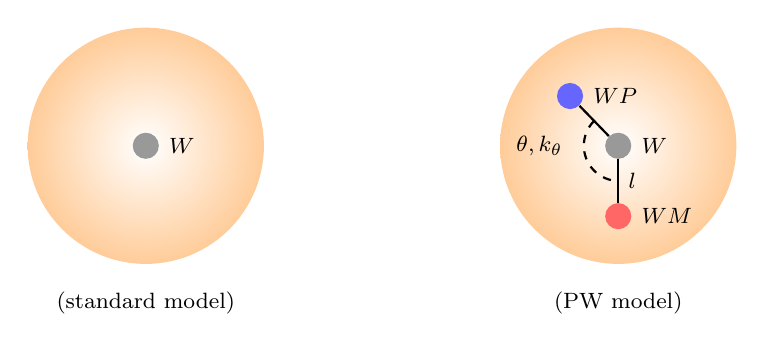
\begin{tikzpicture}
		%\draw[gray,step=1] (-6,-3) grid (6,3);
		\shade[inner color=white,outer color=orange!40] (-3,0) circle (1.5);
		\node[fill=gray!80, circle, radius=0.4, label=right:\footnotesize$W$] at (-3,0) {};
		\shade[inner color=white,outer color=orange!40] (3,0) circle (1.5);
		\node[fill=gray!80, circle, radius=0.4, label=right:\footnotesize$W$] (W) at (3,0) {};
		\node[fill=blue!60, circle, radius=0.4, label=right:\footnotesize$WP$] (WP) at (2.388, 0.632) {};
		\node[fill=red!60, circle, radius=0.4, label=right:\footnotesize$WM$] (WM) at (3,-0.894) {};
		\draw[thick] (W) -- (WP);
		\draw[thick] (W) -- (WM) node[midway,right]{\footnotesize $l$};
		\draw[dashed,thick] (2.694,0.316) arc [start angle=135, end angle=270, x radius=0.447, y radius=0.447];
		\node[] at (2,0) {\footnotesize$\theta,k_\theta$};
		\node[] at (-3,-2){\footnotesize (standard model)};
		\node[] at (3,-2){\footnotesize (\acs{PW} model)};
	\end{tikzpicture}
	\caption{Schematic representation of the \acs{PW} bead. Shaded orange spheres correspond to the Van der Walls radii of the central neutral particle $W$. The blue particle is the positively charged while the red is the negatively charged.}
	\label{fig:PW}
\end{figure}

In the same fashion of the \martini philosophy, Yesylevskyy \etal\, \cite{PW} have developed a \acf{PW} model that better describe the real behavior of water. As before four water molecules is associated to one \ac{PW} bead. The new water bead actually consists of three particles instead of one in the standard \martini model. 
In figure~(\ref{fig:PW}) the topology of the \ac{PW} and a comparison between the old model is shown. The central particle $W$ is neutral and interacts with other particles in the system with only Lennard--Jones potential, just like the standard water bead thus as a $P_4$ \martini bead (see figure~(\ref{fig:martiniInteractions}) for the interactions matrix). There are two additional particles, namely $WP$ and $WM$, that are bound to the central particle and carry a positive and negative charge $|q| = 0.46\mathsf{e}$ respectively, where $\mathsf{e} = 1.60217653(14) \cdot 10^{-19}$~C is the unit electron charge. They interact with other particles in the system by the Coulomb interaction only. The bonds $W-WP$ and $W-WM$ are constrained to have a fixed distance $l = 0.14$~nm. 
The electrostatic interaction between $WP$ and $WM$ inside the same bead are exclude thus they are transparent toward each other and they can rotate around the $W$ particle. As a consequence the dipole momentum of the water bead depends on the relative angular position $\theta$ of $WP$ and $WM$: It can vary from zero ($\theta = 0$), to $2ql$ ($\theta = \pi$). A harmonic angle potential with equilibrium angle fixed to $\theta_0 = 0$ and a force constant $k_\theta = 4.2$~kJ/(mol$\cdot$rad$^2$) is added to control the rotation of $WP$ and $WM$ particles around the $W$ particle so to adjust the distribution of the dipole momentum. The value of the equilibrium angle is consistent with the fact that in an apolar medium the total dipole momentum of a water molecule is zero. 
Since in this model the screening and polarization effects are treated explicitly the global dielectric constant is then reduced from $\varepsilon_r = 15$, used in the standard \martini, to $\varepsilon_r = 2.5$. Moreover, since the \ac{PW} beads attract each other stronger then the standard water beads because of additional electrostatic interactions the strength $\epsilon_{WW}$ of the Lennard--Jones interaction between $W$ particles must be reduced. They found that change the Lennard--Jones strength from an $I$ level to an $III$ level can do the trick (see table~(\ref{tab:martiniEpsilon}) for the various interaction levels). While $\sigma$ remains set to $0.47$~nm.

The parametrization of $q$, $k_\theta$ and $\epsilon_{WW}$ are obtained, in addition to the basic target properties of the \martini \ac{FF}, also trying to reproduce the dielectric constant, density and dipole momentum of a pure water phase. For a more details about the parameterizations and testing methods the reader is addressed to the article by Yesylevskyy \etal\,\cite{PW}. An important question is the use of the \ac{PME} method to treat the long range electrostatic interaction. The authors found that, despite the loss of performance, in addition to the \ac{PW} model, the use of the \ac{PME} method contributes to a more realistic description of the processes involved in a biomolecular environments. In particular, some interesting results of utility for this thesis work, concern a better description of some properties of lipid membranes. One is the translocation of charged ions through a lipid bilayer that is described in a more realist detail: The authors found that the simulations with \ac{PW} and \ac{PME} are approaching the atomistic results better then the standard \martini \ac{FF}. Another important phenomenon about lipid membranes consist in the electroporation of membrane by \ac{PW} beads due to an electric field across the membrane (for example, created by a cross membrane ions imbalance) and, relented to this, the translocation of ions across the membrane helped by a so called ``\textit{water finger}'' a water defect inside the membrane that seems to be the trigger of the ions translocation. Such phenomenons are clearly evident in atomistic simulation however never occurred using the standard \martini \ac{FF} thus the importance to use the \ac{PW} model together with \ac{PME} method.
%Despite this the loss of performance is clearly related to the fact that \ac{PW} increase by a factor $\times 3$ the number of particles in the system related to water.

%\subsection{Applications}

\subsection{Limitations of MARTINI FF}
As we have seen in~\ref{sec:CGModel} the \ac{CG} \acp{FF} are computationally advantages, however a price has to be paid. Although the \martini \ac{FF} is still a finer \ac{CG} \ac{FF}, some limitations are shared with other \ac{CG} models at a fundamental level, such as the chemical and spatial resolution, which are both limited compared to atomistic models. One of the most important question is the \ac{DOF} reduction: This affects the entropy of the system which is underestimated and, as consequence of the \martini parameterizations, also the balance between enthalpy is not correct described. Since the \martini model is built with the constraint that the partitioning free energy $\Delta G = \Delta H - T\Delta S$ must be conserved with the atomistic case, together with an intrinsic loss of entropy, the enthalpic contribution must decrease with respect to the atomistic model\footnote{If a $NVT$ ensemble is used the correct potential is $\Delta A = \Delta U - T\Delta S$, thus the incorrect balance is between the internal energy and the entropy.}. Moreover this mean that the temperature dependence of a \ac{CG} model is a priori not correct, anyway this is not our case since we use only a $NVT$ or a $NPT$ ensemble with an external thermostat coupling.

Another consequence of \ac{CG} \acp{FF} is related to the \ac{PEF} that becomes smoother respect to the atomistic case. This effectively results in more sampling of the energy landscape in a given time period, speeding up the kinetics of the system and allowing the use of an higher time steps with longer simulation times. However the speed--up is not easily predictable and is not likely to be the same for different systems and maybe it is dependent on the type of molecule. Nevertheless for the \martini \ac{FF} an average scaling factor of $4$, based on lateral diffusion coefficients of lipids in membranes, is commonly used, of course with some care. Another smaller source of errors is due to the choice of masses: Since ensemble properties is not affected by particles mass, in order to increase the efficiency, all the \martini beads have the same mass of $72$~amu. This leads in some uncertainty in the dynamics of the system making the time scaling for different beads non--trivial.

A problem involving the Lennard--Jones potential as a model of Van der Waals interaction in \martini, is that the steep repulsion leads to an over--structuring of fluids compared to atomistic models. The direct and most evident implication is the melting point of the water that is $290 \pm 5$~K. A practical partial solution is the use of the so called ``anti--freeze'' particles named BP$_4$ type. The Lennard--Jones interaction between these particles and water is modified with a slightly larger Van der Waals radius parameter, $\sigma = 0.57$~nm and a stronger interaction to be a level $O$ (see table~(\ref{tab:martiniEpsilon}) for the interaction level). Marrink \etal\, suggest that a mole fraction of $n_{\text{af}} = 0.1$ is sufficient to prevent freezing without affecting the other properties of water. Some other properties of water are not accurate described such us the surface tension of air/water interface that leads in problem to water/oil interfaces formation. Using the \ac{PW} model these properties improve slightly. For a more comprehensive discussion about the limitations of the \martini \ac{FF} the reader is addressed to the review by Marrink \etal\, \cite{MartiniReview}.

\section{Advanced sampling methods}
	\subsection{Metadynamics}

	\subsection{Umbrella sampling} %Molecular Modelling, 581


%Manuale GROMACS 3.17.5 PP/PME ranks
